\section{Experimental methods}

\subsection{Potential step method}

This is a way to evaluate the current potential characteristic of a cell by using a particular apparatus called \textbf{potentiostat} or \textbf{galvanostat}. The idea is to add into the cell a third electrode along with the reference and working one, called \textbf{counter electrode} (CE), in order to prevent potential variations due to current flowing through the RE. Still, the potential of the cell is evaluated by the difference in potential of the RE and WE, but the other one allows us to control such a potential along with the current that is circulating inside the cell.
\begin{figure}[t]
    \centering
    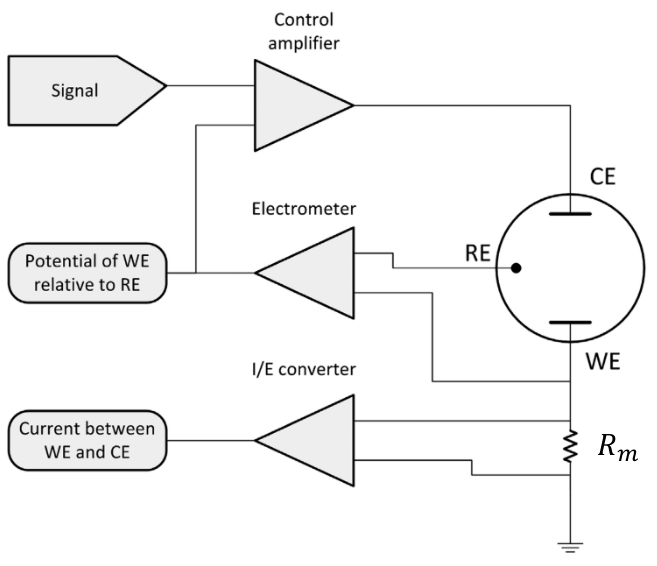
\includegraphics[width=0.4\textwidth]{Immagini/Potentiometer.png}
    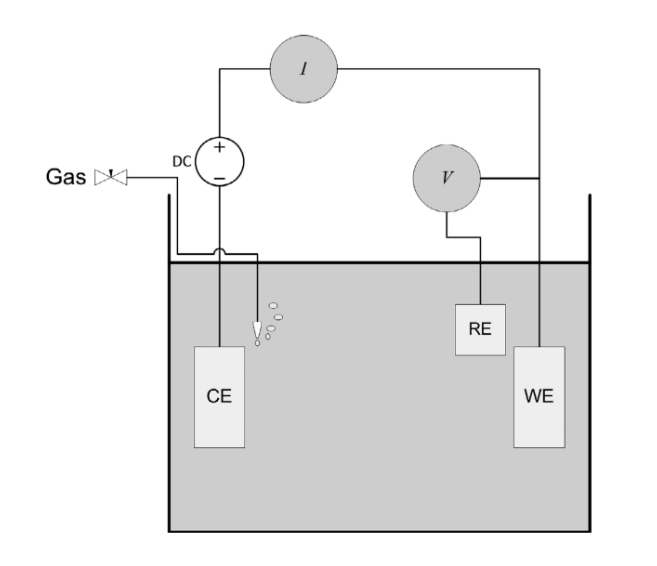
\includegraphics[width=0.4\textwidth]{Immagini/CellaTreElettrodi.png}
    \caption{
        Graphical representation of the working device used in this particular method, both in the circuit part and the implementation of the cell.
    }
    \label{eq:PotGal}
\end{figure}
In particular, we can have a look at \figref{eq:PotGal} to see effectively how the setup works, basically you have the electrometer that evaluates $E_{WE} - E_{RE}$ and passes that value to the control amplifier that controls if that potential is equal to the signal value that we want and generates a current in the CE in order to lower or increase the potential of the cell accordingly. In this way we are able to control the cell potential while monitoring the current that is passing through it using the I/E converter part of the circuit, therefore collecting the I vs E characteristic.

Inside a general experiment of this type usually one applies a potential $E_1$ where Faradic processes are not occurring so that no current basically flows inside the circuit. Then, the potential is increased to $E_2$ inside the Faradic region allowing for the system to reach the mass-limited current regime with $J_L$ that decrease over time due the Nernst layer becoming thicker. We can so monitor the evolution of the current over time setting the $t=0$ moment as the one where we switch from $E_1$ to $E_2$ so that we expect an evolution of the current of the type
\begin{align}
    &E(t) = \begin{cases}
        E_1 & t_i < t < 0\\
        E_2 & t > 0
    \end{cases}, &i(t) = \begin{cases}
        \frac{E}{R_S}e^{-\frac{\abs{t}}{R_SC_{dl}}} & t_i < t < 0\\
        nFAC_{O,b}\sqrt{\frac{D_O}{\pi t}} & t > 0
    \end{cases}.
\end{align}
Where before the switch the current is the one of the RC circuit, while in the Faradic region is the equation of the limiting current. In this way we can decide a time $\tau$ at which we are going to collect the current for a certain potential $E_2$ and then after collecting $i(\tau)$ for several values we can reconstruct the characteristic in order to fit it with the Butler-Volmer model 
\begin{equation}
    i = i_0\left[ e^{-\alpha\frac{F\eta}{RT}} - e^{-(\alpha - 1)\frac{F\eta}{RT}} \right],
\end{equation}
which can give information about $\alpha$ or $i_0$.

Another possibility is to perform a \textbf{Linear sweep} where the potential is changed over time not in a stepped way but using $E = E_i - \nu t$ so that we can control $i(E)$ in time so that we obtain several regions that allows us to have information:
\begin{itemize}[align=left, leftmargin=*]
    \item[$E\ll E^0$]: mainly non-Faradic current due to charging of double layer;
    \item[$E\sim E^0$]: reduction starts, thus $C_{O, x=0}$ decrease while $C_{R, x=0}$ increase;
    \item[$E=E^{peak}$]: the reactant is fully consumed at the surface and mass-transfer reaches a maximum rate due to the maximum concentration gradient;
    \item[$E > E^{peak}$]: the depletion layer starts to increase, therefore the current decrease, stabilizing to a current depending on the steady state thickness.
\end{itemize}
If we assume Nernstian conditions the current-potential relation can be solved analytically in order to obtain the energy of the peak and the current as
\begin{align}
    &E^{peak} = E_{1/2} - 1.109\frac{RT}{nF}, &i^{peak} = (2.69\times 10^5)AC_{O,b}\sqrt{n^3 D_O\nu},
\end{align}
allowing to find out information on both number of electrons involved in the reaction, $n$, and diffusion coefficient, $D_O$. Nevertheless, in this case the evaluation has a complication due to the presence of a resistance inside the solution, $R_{cell}$, that generate an internal drop of potential proportional to the current so that we shall account for it as
\begin{equation}
    E_{cell} = E_{WE} - E_{CE} - iR_S.
\end{equation}
Therefore, a correction needs to be added to the measurements, and we need also to be careful since Faradic and non-Faradic components of the current are summed in the final result so that remembering how $i_F \propto \sqrt{\nu}$ at LSV peak and $i_c \propto \nu$ if the scanning rate, $\nu$, is too high the $i_c$ will dominate on $i_F$ having so a lower peak difficult to see. Another problem is that if we have a precision, sett by the scanning rate, comparable with the bias $i_{tot}R_u$ the sweep will not be truly linear and the curve will flatten for more negative values of $E$ not allowing us to identify the peak. Thus, we need to carfully tune $\nu$, also because having how $i^{peak} \propto \sqrt{\nu}$ we have that higher the scan rate the more $E^{peak}$ will be shifted being a function of $\nu$ as well.

The last way we have seen in order to experimentally study the evolution of the cell potential was the \textbf{cyclic voltammetry}, the idea is to perform two linear sweep right one after the other in opposite directions. In particular, you want to increase the potential reaching the LSV to then quickly turn back and return to the starting one. 
\begin{figure}[t]
    \centering
    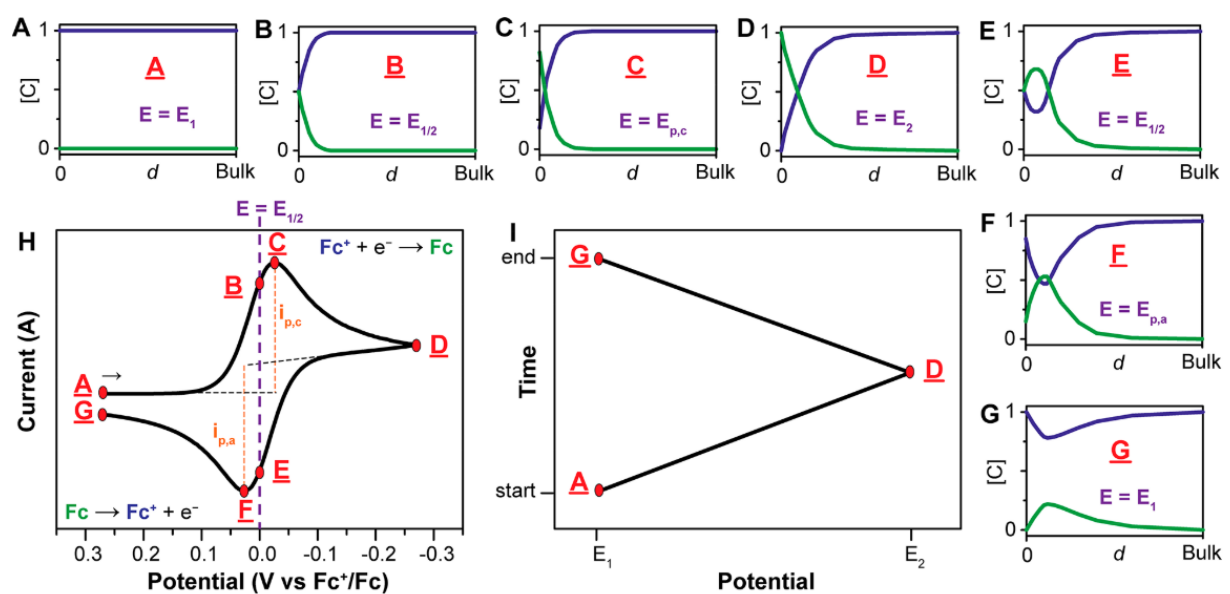
\includegraphics[width=0.8\textwidth]{Immagini/CyclicVoltam.png}
    \caption{
        Representation of the potential, current and concentration inside a cyclic voltammetry experiment showing how the final form of the caratteristic is a loop like form that is influenced by the slowness of diffusion in order to perfectly return to the initial point.
    }
    \label{fig:CyclicVoltam}
\end{figure}
This can be seen in \figref{fig:CyclicVoltam} where we can see how the concentration gradient changes inside the material and turns back during the process, still not becoming the initial one due to slowness of diffusion. Still, in this data we can see both peaks for both forward and backward reactions inside the system giving us information on both peaks positions that allows us to evaluate the formal potential
\begin{equation}
    E_{pc} - E_{pa} = E_{1/2} \approx E^0.
\end{equation} 
Then we can also give an estimate of the reversibility of the reaction by evaluating the ratio $i_{pa}/i_{pc}$ related to the reaction rate ones, and also to the electrochemical reversibility, which is proportional to $\Delta E_p$ having that in particular the following is true 
\begin{align}
    &\Delta E_p^{rev} = 2.3\frac{RT}{nF}, &\Delta E_p^{non-rev} > 2.3 \frac{RT}{nF}.
\end{align}
To make an example of how this works one can take a reaction of the following type
\begin{equation}
    \ce{O + e^-}\rightleftharpoons \ce{R -> Z}, 
\end{equation}
where the first is reversible while the second not. The form of the CV cycle is highly dependent on the rate, $k_c$, of the second reaction: if is small is like nothing happens and the cycle is normal, but if it's high the reaction is not fully able to come back and the back process curve flattens out. This also allows to evaluate a so-called \textbf{reversibility parameter} $\alpha$ that is not sad how to compute it really, but I will trust the prof on words.